 % Implement the Jacobi Method.
Write a function that accepts a matrix $A$, a vector $\b$, a convergence tolerance \li{tol}, and a maximum number of iterations \li{maxiters}.
Implement the Jacobi method using (\ref{eq:jacobi-method}), returning the approximate solution to the equation $A\x = \b$.

Run the iteration until $\|\mathbf{x}^{(k-1)} - \mathbf{x}^{(k)}\|_{\infty} <$ \li{tol}, and only iterate at most \li{maxiters} times.
Avoid using \li{la.inv()} to calculate $D^{-1}$, but use \li{la.norm()} to calculate the vector $\infty$-norm $\|\x\|_\infty = \sup{|x_i|}$.

% \begin{lstlisting}
% >>> from scipy import linalg as la
%
% >>> x = np.random.random(10)
% >>> la.norm(x, <<ord>>=np.inf)          # Use la.norm() for ||x||.
% 0.74623726404168045
% >>> np.<<max>>(np.<<abs>>(x))               # The equivalent in NumPy for ||x||.
% 0.74623726404168045
% \end{lstlisting}

Your function should be robust enough to accept systems of any size.
To test your function, generate a random $\b$ with \li{np.random.random()} and use the following function to generate an $n\times n$ matrix $A$ for which the Jacobi method is guaranteed to converge.
Run the iteration, then check that $A\x^{(k)}$ and $\b$ are close using \li{np.allclose()}.

\begin{lstlisting}
def diag_dom(n, num_entries=None):
    """Generate a strictly diagonally dominant (n, n) matrix.
    Parameters:
        n (int): The dimension of the system.
        num_entries (int): The number of nonzero values.
            Defaults to n^(3/2)-n.
    Returns:
        A ((n,n) ndarray): A (n, n) strictly diagonally dominant matrix.
    """
    if num_entries is None:
        num_entries = int(n**1.5) - n
    A = np.zeros((n,n))
    rows = np.random.choice(np.arange(0,n), size=num_entries)
    cols = np.random.choice(np.arange(0,n), size=num_entries)
    data = np.random.randint(-4, 4, size=num_entries)
    for i in range(num_entries):
        A[rows[i], cols[i]] = data[i]
    for i in range(n):
        A[i,i] = np.<<sum>>(np.<<abs>>(A[i])) + 1
    return A
\end{lstlisting}

Also test your function on random $n \times n$ matrices.
If the iteration is non-convergent, the successive approximations will have increasingly large entries.

\label{prob:jacobi}

Modify your Jacobi method function in the following ways.
\begin{enumerate}
    \item Add a keyword argument called \li{plot}, defaulting to \li{False}.
    \item Keep track of the absolute error $\|A\mathbf{x}^{(k)} - \mathbf{b}\|_{\infty}$ of the approximation at each iteration.
    \item If \li{plot} is {True}, produce a lin-log plot (use \li{plt.semilogy()}) of the error against iteration count.
    Remember to still return the approximate solution $\x$.
\end{enumerate}
If the iteration converges, your plot should resemble the following figure.

\begin{figure}[H]
    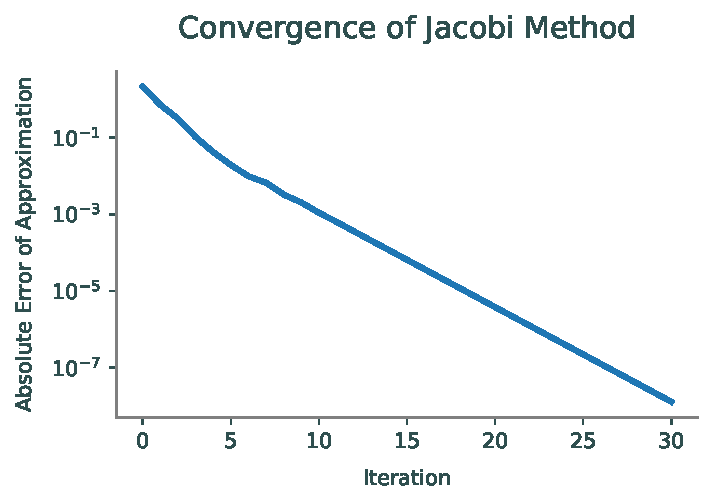
\includegraphics[width=.7\textwidth]{figures/jacobi_convergence.pdf}
\end{figure}

\label{prob:plot-iterative-convergence}
 % Implement Gauss-Seidel.
Write a function that accepts a matrix $A$, a vector $\b$, a convergence tolerance \li{tol}, a maximum number of iterations \li{maxiters}, and a keyword argument \li{plot} that defaults to \li{False}.
Implement the Gauss-Seidel method using (\ref{eq:gauss_seidel}), returning the approximate solution to the equation $A\x = \b$.

Use the same stopping criterion as in Problem \ref{prob:jacobi}.
Also keep track of the absolute errors of the iteration, as in Problem \ref{prob:plot-iterative-convergence}.
If \li{plot} is \li{True}, plot the error against iteration count.
Use \li{diag_dom()} to generate test cases.

\begin{warn} % Arrays are mutable!
Since the Gauss-Seidel algorithm operates on the approximation vector in place (modifying it one entry at a time), the previous approximation $\x^{(k-1)}$ must be stored at the beginning of the $k$th iteration in order to calculate $\|\x^{(k-1)} - \x^{(k)}\|_\infty$.
Additionally, since NumPy arrays are mutable, the past iteration must be stored as a \textbf{copy}.

\begin{lstlisting}
>>> x0 = np.random.random(5)        # Generate a random vector.
>>> x1 = x0                         # Attempt to make a copy.
>>> x1[3] = 1000                    # Modify the "copy" in place.
>>> np.allclose(x0, x1)             # But x0 was also changed!
<<True>>

# Instead, make a copy of x0 when creating x1.
>>> x0 = np.copy(x1)                # Make a copy.
>>> x1[3] = -1000
>>> np.allclose(x0, x1)
<<False>>
\end{lstlisting}
% It is good practice in most iterative methods to record a copy of $\x^{(k-1)}$ at the beginning of the $k$th iteration.
\end{warn}

\label{prob:gauss_seidel}
 % Sparse implementation of Gauss Seidel.
The Gauss-Seidel method is faster than the standard system solver used by SciPy's \li{la.solve()} if the system is sufficiently large and sufficiently sparse.
For $n=5,6,\ldots,11$, generate a random $2^n \times 2^n$ matrix $A$ using \li{diag_dom()} and a random $2^n$ vector $\b$.
Time how long it takes to solve $A\x = \b$ using your Gauss-Seidel function from Problem \ref{prob:gauss_seidel}, and how long it takes to solve using \li{la.solve()}.
Make a log-log plot of the times against the system size.
 % Gauss-Seidel with Sparse matrices.
Write a new function that accepts a \textbf{sparse} matrix $A$, a vector $\b$, a convergence tolerance \li{tol}, and a maximum number of iterations \li{maxiters} (plotting the convergence is not required for this problem).
Implement the Gauss-Seidel method using (\ref{eq:gauss_seidel}), returning the approximate solution to the equation $A\x = \b$.
Use the usual stopping criterion.

The Gauss-Seidel method requires extracting the rows $A_i$ from the matrix $A$ and computing $A_i\trp\x$.
There are many ways to do this that cause some fairly serious runtime issues, so we provide the code for this specific portion of the algorithm.

\begin{lstlisting}
# Get the indices of where the i-th row of A starts and ends if the
# nonzero entries of A were flattened.
rowstart = A.indptr[i]
rowend = A.indptr[i+1]

# Multiply only the nonzero elements of the i-th row of A with the
# corresponding elements of x.
Aix = A.data[rowstart:rowend] @ x[A.indices[rowstart:rowend]]
\end{lstlisting}

To test your function, cast the result of \li{diag_dom()} as a sparse matrix.

\begin{lstlisting}
>>> from scipy import sparse

>>> A = sparse.csr_matrix(diag_dom(50000))
>>> b = np.random.random(50000)
\end{lstlisting}
 % SOR
Write a function that accepts a sparse matrix $A$, a vector $\b$, a relaxation factor $\omega$, a convergence tolerance \li{tol}, and a maximum number of iterations \li{maxiters}.
Implement SOR using (\ref{eq:sor}), compute the approximate solution to the equation $A\x = \b$.
Use the usual stopping criterion.
Return the approximate solution $\x$ as well as the number of iterations computed.
\\ (Hint: this requires changing only one line of code from the sparse Gauss-Seidel function.)
\label{prob:sor}

Write a function that accepts an integer $n$, a relaxation factor $\omega$, a convergence tolerance \li{tol} that defaults to $10^{-8}$, a maximum number of iterations \li{maxiters} that defaults to $100$, and a bool \li{plot} that defaults to \li{False}.
Generate and solve the corresponding system $A\u = \b$ using Problem \ref{prob:sor}.
Also return the number of iterations computed.
\\ (Hint: see Problem \ref{prob:sparse-construction} of the Linear Systems lab for the construction of $A$.
Also, \li{np.tile()} may be useful for constructing $\b$.)

If \li{plot=True}, visualize the solution $\u$ with a heatmap using \li{plt.pcolormesh()} (the colormap \li{"coolwarm"} is a good choice in this case).
This shows the distribution of heat over the hot plate after it has reached its steady state.
Note that the $\u$ must be reshaped as an $n\times n$ array to properly visualize the result.
\label{prob:finite-difference-setup}

To demonstrate how convergence is affected by the value of the relaxation factor $\omega$ in SOR, run your function from Problem \ref{prob:finite-difference-setup} with $\omega = 1,\ 1.05,\ 1.1,\ \dots , 1.9, 1.95$ and $n = 20$.
Plot the number of computed iterations as a function of $\omega$.
Return the value of $\omega$ that results in the least number of iterations.

Note that the matrix $A$ from Problem \ref{prob:finite-difference-setup} is not strictly diagonally dominant.
However, $A$ is positive definite, so the algorithm will converge.
Unfortunately, convergence for these kinds of systems usually requires more iterations than for strictly diagonally dominant systems.
Therefore, set \li{tol=1e-2} and \li{maxiters=1000}.

Recall that $\omega = 1$ corresponds to the Gauss-Seidel method.
Choosing a more optimal relaxation factor saves a large number of iterations.
This could translate to saving days or weeks of computation time while solving extremely large linear systems on a supercomputer.

Laplace's equation is used to model steady-state heat flow on a square plate.
The plate can be approximated by a matrix, where each entry of the matrix represents the average temperature over a small square portion of the plate.
Suppose the plate starts at $0^\circ$ Celsius everywhere except on the east and west boundaries, which are held at a constant temperature of $100^\circ$.
In addition, the north and south boundaries are held constant at $0^\circ$.

\[
U = \left[\begin{array}{ccccc}
\textcolor[rgb]{0.,0.,1.}0 & \textcolor[rgb]{0.,0.,1.}0 & \textcolor[rgb]{0.,0.,1.}\cdots & \textcolor[rgb]{0.,0.,1.}0 & \textcolor[rgb]{0.,0.,1.}0\\
\textcolor[rgb]{1.,0.,0.}{100} & 0 & \cdots & 0 & \textcolor[rgb]{1.,0.,0.}{100}\\
\textcolor[rgb]{1.,0.,0.}\vdots & \vdots & \ddots & \vdots & \textcolor[rgb]{1.,0.,0.}\vdots \\
\textcolor[rgb]{1.,0.,0.}{100} & 0 & \cdots & 0 & \textcolor[rgb]{1.,0.,0.}{100}\\
\textcolor[rgb]{0.,0.,1.}0 & \textcolor[rgb]{0.,0.,1.}0 & \textcolor[rgb]{0.,0.,1.}\cdots & \textcolor[rgb]{0.,0.,1.}0 & \textcolor[rgb]{0.,0.,1.}0\\

\end{array}\right]
\]

The non-boundary, interior portion of the matrix (with black text) can be accessed with the slice \li{U[1:-1,1:-1]}.
To find the steady state of the hot plate, set each entry of the interior of $U$ equal to the average of its 4 immediate neighbors (the entries above, below, and to the left and right).
This step should take only \emph{one line} and should be based entirely on array slicing.

Continue updating the interior entries of $U$ until they stop changing significantly.
The entire procedure is summarized in Algorithm \ref{alg:jacobi}.

Hint: The slice \li{U[:-2,1:-1]} references the upper neighbors of the interior points of $U$ and \li{U[1:-1,2:]} references the right neighbors. How can you reference the lower and left neighbors?

Use the following code to visualize your results.
%% This does 3D visualization, but it's easier (and better) as a heat map.
% from mpl_toolkits.mplot3d import Axes 3D

%     x, y = np.linspace(0, 1, n), np.linspace(0, 1, n)
%     X, Y = np.meshgrid(x, y)
%     fig = plt.figure()
%     ax = fig.gca(projection='3d')
%     ax.plot_surface(X, Y, U, rstride=5)
%     plt.show()

\begin{lstlisting}
from matplotlib import pyplot as plt

def jacobi(n=100, tol=1e-8):

    # Perform the algorithm, storing the result in the array 'U'.

    # Visualize the results.
    plt.imshow(U)
    plt.show()
\end{lstlisting}

This Jacobi iteration is a \emph{finite difference method}, and is similar to many of the methods that we will use to find numerical solutions to differential equations in Volume IV.
